\section{Methods and implementation}\label{sec:methods}
Due to the complexity of the Sokoban problem, blindly expanding nodes in hopes of finding the solution will most likely fail on the majority of maps. This rules out the usage of un-informed search methods, such as depth-first search - DFS (expand every first child node) and breadth-first search - BFS (expand every node at a certain depth) as feasible methods of solving Sokoban puzzles. Un-informed algorithms are characterized by the lack of ``judgement'' in making node expansion decisions. They simply follow a fixed pattern, as mentioned above, that has no correlation to the values of the nodes.

The concept of informed-search emerges from the need of a better method and the general form of informed-search algorithms is the best-first search (Best-FS). As its name states, best-first search is a method that expands the most promising node first, according to a predefined criteria, a score. This score is given to every map and is based on heuristics, which are  strategies using readily accessible information to control problem-solving processes in man and machine \cite{pearl1984heuristics}. Heuristic methods are used to speed up the process of finding a satisfactory solution, where an exhaustive search is impractical. In our case, some good heuristics, which contribute to the score of a map, are: the number of boxes on goal positions, the distance from the boxes to the goals, the distance from the player to the closest box.

Another important aspect of Sokoban maps is the existence of deadlocks. These are states that cannot lead to a solution. Deadlocks that are inherent to a map, such as boxes being stuck in a corner, are easily avoidable. Other types of deadlocks are more difficult to manage (for example having 2 boxes at the ends of a tunnel). A good solver must be aware of as many deadlocks as possible, in order to properly prune the search tree and not consider branches that are not able to produce a solution. Some trivial deadlock positions are marked in figure \ref{fig:sokoban_map}, using a green X symbol. 

\begin{figure}[h]
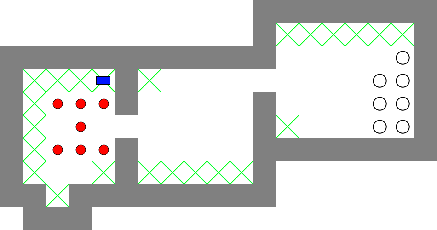
\includegraphics[width=\columnwidth]{./images/deadlocks.png}
\caption{Sokoban map with marked deadlocks}
\label{fig:sokoban_map}
\end{figure}

\subsection{Architecture}
Several key components can be identified in the architecture, as visualized in figure \ref{fig:architecture}. While interaction is subtly more complex in places than the diagram implies, in general they can be attributed to the following components:
\begin{enumerate}
	\item \textbf{Client} handles communication with the Sokoban server. This loads the textual representation of the map, and sends the proposed textual representation of the solution back to the server.
	\item \textbf{Core} initializes the client, then creates a Map and Solver object. The core acts as a process controller, ensuring that each component receives the information it requires.
	\item \textbf{Map} object representation of the loaded map. Map objects can be manipulated, in that the location of the player and boxes can change, and keep track of those changes to provide a move history. They also simplify other tasks through deadlock detection and state checking.
	\item \textbf{Heuristics} based on a certain map, the Heuristics calculate a score to assign to that map which corresponds to the state of that map, solver-wise. The closer a map gets to being solved, the higher its heuristics score will be.
	\item \textbf{Solver} any solver extends a base Solver class, which loads information from the core and heuristics and returns a solution when it is found.
	\item \textbf{Solver Implementations} Each Solver implementation runs in a separate thread and performs the necessary operations to solve the loaded Map. Actual implementation of each solver is discussed in more detail in section \ref{solvers}.
\end{enumerate}

\begin{figure*}
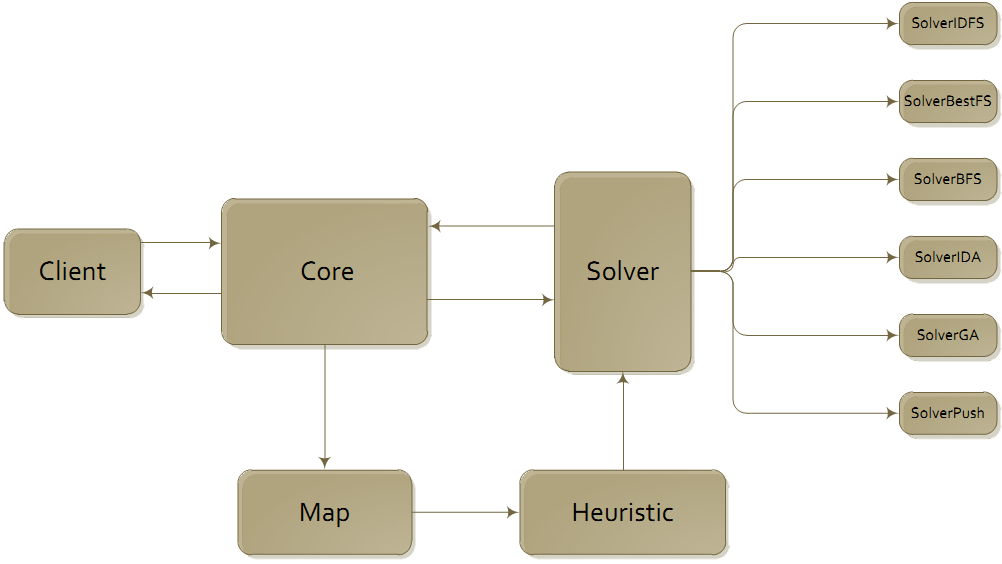
\includegraphics[width=2.1\columnwidth]{./images/architecture.png}
\caption{ Architectural components and workflow}
\label{fig:architecture}
\end{figure*}




\subsection {The map}
The map is received as a string of characters and is parsed into a matrix of bytes, where there is an assigned bit to each of the following: player, box, wall, goal, deadlock. Also, if 2 or more of the above mentioned entities are not mutually exclusive (the player and a goal for example), there is a value assigned to their combination.  These values can then be manipulated every time a move is performed, in order to produce the resulting map.

The first action taken after the map is parsed, before attempting to solve it, is to mark the squares where if a box is pushed, the map would become deadlocked. These positions are the corners and the sides of the walls connecting the corners. No move that pushes a box onto these positions is allowed.

Later on in the process of moving the player, the map is checked for other types of deadlocks, such as 2 boxes being next to each other against a wall, a position from which they cannot be moved. If such situations occur, the solvers discard the current branch of the search tree, saving time.

\subsection{Heuristics}\label{Heuristics}
Heuristics are used in informed-search algorithms to help with ordering the states (maps in our case), prior to expanding. We used heuristics by assigning an integer value to each map. The higher this value is, the better the map becomes and the likelihood of choosing it for expanding grows. The map's score is directly proportional to the number of boxes that are on goal positions and inversely proportional to the distances from the boxes to the goals and from the player to the nearest box. That translates to: it's good to have as many boxes on goals, it's good to have a short distance from the boxes to the goals, it's good to have a short distance from the player to the closest box.

\subsection{Solvers}\label{solvers}
\subsubsection{Breadth-First Search}
Breadth-First Search (BFS) is a graph search algorithm that aims to examine all nodes through exhaustive exploration. The method is trivial and frequently used. BFS uses a FIFO(First In, First Out) queue which stores nodes that need to be expanded. Each visited node is placed in a separate  list, called a closed set, and is not examined again. The algorithm ends successfully when it finds a solution node, without taking into account if it is the best one.

A basic implementation of this algorithm is used to solve a Sokoban puzzle. Each node represents a map in a particular state. When the algorithm runs, it expands the nodes based on the move performed by the player. BFS stops when a node in which all the boxes are placed on the goal positions is found. 

\subsubsection{Depth-First Search}
The depth-first search algorithm is one of the most basic tree search algorithms available. Though many variants exist (see for example Nishihara and Minamide, 2004 \cite{nishihara2004depth}), most share common properties: a low cost in memory (since only the current branch needs to be tracked) and completeness, if the solution is within the maximum search depth and the branching factor is finite, conditions that are met in the Sokoban puzzle case.

\subsubsection{Best-First Search}
Best-FS is a heuristic based search algorithm. A node is expanded if it has the best score of all the nodes. The score is calculated by an evaluation function f(n). Best-FS uses a priority queue in order to obtain the best node while the algorithm runs and a closed set in order to avoid repeated states and cycles. It is a greedy algorithm and does not always return the optimal solution. However, it gives fast results when it finds a very good solution.\cite{korf1993linear}

We used an implementation of Best-FS as the main solver of a Sokoban puzzle. Each state is represented by an object(NewNode) which contains a map and the score of the map. The nodes are expanded based on an evaluation function which is described above\ref{Heuristics}. In each turn we reorder the expanded nodes in a priority queue and we choose the node with the highest value. The agent chooses moves which have smaller distances between the player position and the boxes or the boxes' positions and the goals. In this way, it finds an optimal way to reach the boxes quickly and afterwards push them onto the goal positions.

\subsubsection{Iterative-Deepening A* Search}
IDA* is an optimization of the A* algorithm which uses iterative deepening to keep the memory usage lower than in A*. Traditionally, A* uses best-first search with a heuristic function linked to the distance from the start position to the current position. It finds the least-cost path from an initial node to a goal node.\cite{stout1996smart}

In Sokoban puzzles we used IDA* in order to find the best path to a goal position. The heuristic that we used is based on Manhattan distances between the player and the boxes and between the boxes and the goal positions. The algorithm increases the depth of searching until it can find a solution state.

\subsubsection{Genetic Algorithm}
Genetic Algorithms belong to the class of Evolutionary Algorithms, which are based on evolutionary processes like mutation, cross-over and survival of the fittest. They have been used in search, optimization and machine learning problems for decades \cite{goldberg1989genetic}. In fact, solving so called motion planning problems with Genetic Algorithms has been researched before \cite{amosgenetic}\cite{coldridge2010genetic}.

A basic genetic algorithm is employed to solve the Sokoban puzzle. Each "individual" consists of a series of moves, each move denoted by one of the four possible directions (Up, Down, Left, Right). Impossible moves, those who would result in either the player or a box moving through a wall or a box, are ignored. The fitness of each individual is determined through the heuristics score of the resulting map after all legal moves have been applied, see section \ref{Heuristics}.

Mutation causes random moves to switch to alternate directions. Since a single change can significantly decrease the fitness of an individual, this mechanism is not used for the top five individuals. These do however participate in cross-over and survival-of-the-fittest to create a new generation, thus propagating their excellent genes to the rest of the population. While this approach does not necessarily yield an optimal solution, nor any solution at all given a certain time limit, it does provide a unique ability to 'stumble upon' a good solution much faster than brute force would allow.

\subsubsection{Push Solver}
The main characteristic of this solver is that the search tree is build based on non-trivial moves (moves which involve a box push).
The fact that this solver disregards trivial movements (moves which do not modify the box locations) makes it capable of solving the same map at a lower depth than other algorithms. The downside of this algorithm is that once the program finds the solution it has to reconstruct the path of trivial moves between box pushes.

Another problem is that the heuristics have to be adapted to prioritize not only moves but also boxes. This algorithm becomes very useful for Sokoban boards where there are plenty of possible player moves but only a few reachable boxes and few possible moves per box.
The way the algorithm works makes it good for this task because it will only expand the possible moves of the reachable boxes keeping the search tree at the minimal depth.

A key aspect implementing this solver is being able to determine efficiently if the player can reach certain board positions. This is achieved with recursion using a function that spreads the influence of the player by calling itself on the surrounding squares until it can't spread any more.